\documentclass{article}
\usepackage{spconf,amsmath,graphicx}
\usepackage{amssymb,mathtools}
\usepackage{graphicx}
\usepackage{listings}
\usepackage{url}
\usepackage{hyperref}
{\scshape}
\graphicspath{ {./images/} }
\DeclarePairedDelimiter{\norm}{\lVert}{\rVert}
\DeclarePairedDelimiter{\abs}{\lvert}{\rvert}
\def\x{{\mathbf x}}
\def\L{{\cal L}}
\title {Element Rank \\[0.5ex] \large Ranking Java Software Classes and Packages using a Multilayer Complex Network-Based Approach}
%
% Single address.
% ---------------
\name{Suresh (M20AIE313), Utkarsh (M20AIE318)}
\author{Carl Capybara\thanks{I never procrastinate} \and Walter Wombat}
\address{IIT Jodhpur}
\begin{document}
%\ninept
%
\maketitle
%
\begin{abstract}
    The software comprehension at the code level is a complex process as it involves the many layers, components, arch& code level design structures, workflow&, etc. Furthermore, the software API documentation, developer comments, and generating component diagrams may not help extensively understand the different software elements. Therefore, the comprehension process at the code level has a lot of complexities. In this work, we will show how the topological structure of software at the class level and package level. First, we use the ElementRank algorithm for ranking at class, and package level, then implement an analytic hierarchy process to weight each layer of multilayer software network and then implement the global weighted page rank for each class.
    
    The outcome of the overall process would help the maintainers better understand code infrastructure in large software systems. In addition, quantifying the class importance with rank would help maintenance personnel with starting points of software comprehension at the code level. Finally, we will apply the proposed algorithm to various open-sourced projects and show how quantifying results help the maintainers. \vspace{2cm}
\end{abstract}
%
\begin{keywords}
PageRanking, Weighted Graph, Multi layer software network
\end{keywords}
%

\newpage

\section{Introduction}
\label{sec:intro}
Understanding Large scale software systems with typical complex interacting elements like packages / classes / interfaces / inheritances / methods / attributes is a time taking process and cause maintenance of the code challenging task. The main objective is to provide the technology which would find the structure and importance of the classes and packages in large complex source code base so that maintenance personal time to understand the code would be reduced and help further to change the code structure better to improve the performance.


\section{Objectives \& Summary}
\label{sec:objectives}
The Element ranking is enhanced formula of Page ranking to get the rank for each element and then aggregate with the Analytical hierarchy process. The weighted page rank value of each element class/package of any layer will be aggregated. 
\textbf{This process involves the steps:}

\begin{itemize}
    \item read the structure of the code and prepare the network layer graphs for each relation
    \item calculate the page rank of element and aggregating the weighted page rank with analytical hierarchy process
\end{itemize}

\textbf{Relations found are:}
\begin{itemize}
    \item Inheritance INR
    \item Implements IMR.
    \item Parameter PAR
    \item Global variable GVR
    \item Method call MCR
    \item Local variable LVR
    \item Return type RTR
\end{itemize}

The relative importance between each relation is taken from the paper $W = (0.034, 0.290, 0.034, 0.034, 0.178, 0.394, 0.034)$

\newpage

\section{Comparison with existing work}
\label{sec:comWork}
The actual page rank algorithm enhanced to consider the weighed graph as below

\begin{itemize}
    \item \textbf{Page Ranking}
        \begin{equation}
            PR(p_i) = \frac{1-d}{N} + d \sum_{p_j \epsilon lnLinks(p_i)} \frac{PR(p_j)}{OutLinks(p_j)}
        \end{equation}
    \item \textbf{Weighted Page Rank}
        \begin{equation}
            \begin{split}
                PR_w(p_i) = \\
                & \frac{(1-d) \times w lnLinks(p_i)}{N} + \\
                & d \sum_{k=1}^{N} w lnLinks(p_k) +  \\
                & d \sum_{p_j \epsilon lnLinks(p_j)} \frac{PR_w(p_j \times w(p_j,p_i))}{wOutLinks(p_j)}
            \end{split}
        \end{equation}
    \item \textbf{Aggregated or Global weighted page rank}
        \begin{equation}
            PR_w^g(p_i) =  \sum_{l = 1}^{o} w_l \times PR_w^l(p_i)
        \end{equation}
\end{itemize}

\newpage

\section{Testing}
\label{sec:test}
As part of algorithm testing, we have taken the java jdk code MPN network to compute the global weighted page ranks.
\subsection{Ranks calculated by our code}
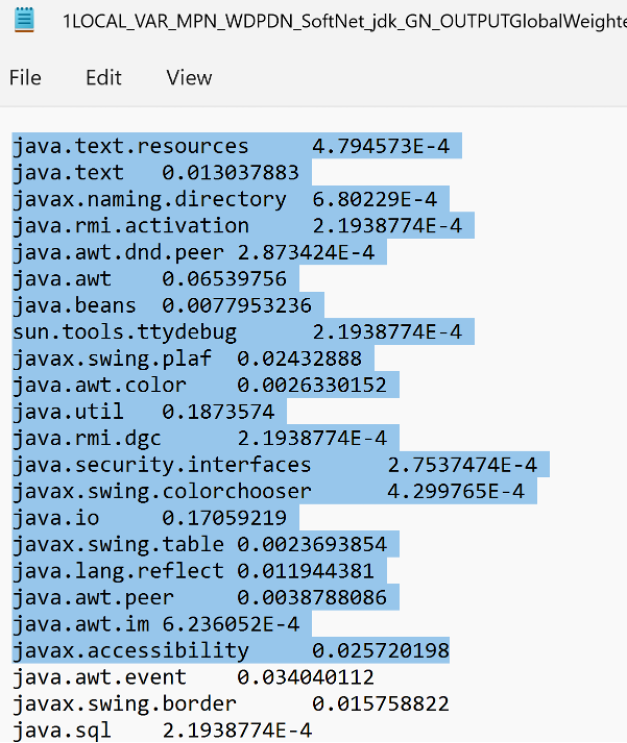
\includegraphics[scale=0.7]{image1.png}

\subsection{original ranks provided for the same data set from paper}
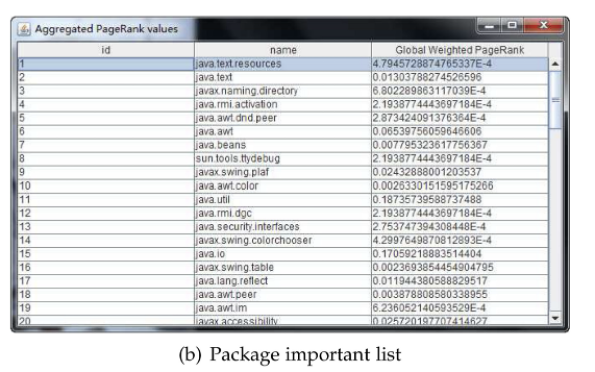
\includegraphics[scale=0.7]{image2.png}


\section{Links}

\begin{itemize}
    \item \href{https://github.com/bojjam1/Assignments}{GitHub Code}
    \item \href{https://drive.google.com/file/d/1rmtP1HgzlxNoUydJNMuBLonglkQYOysS/view?usp=sharing}{Demo Video}
\end{itemize}


\newpage
\section{Summary}
\label{sec:summary}
In this project we have successfully extarcted classes and other packages from java jdk code, applied the algorithim suggested in the pager and have received identical efficiency as that of the paper.

\bibliographystyle{IEEEbib}
\bibliography{strings,refs}

\end{document}
